\section{Additional Results on LSP dataset}
\label{seq:supplemental:lsp}
We provide additional quantitative results on LSP dataset using
person-centric (PC) and observer-centric (OC) evaluation settings.
\subsection{LSP Person-Centric (PC)}
First, detailed performance analysis is performed when evaluating
various parameters of $\rcnn$ and results are reported using
PCK~\cite{sapp13cvpr} evaluation
measure. Then, performance of the proposed $\rcnn$ and $\dense$ part
detection models is evaluated using strict PCP~\cite{Ferrari:2008:PSS}
measure.

\myparagraph{Detailed $\rcnn$ performance analysis (PCK).} Detailed
parameter analysis of $\rcnn$ is provided in
Tab.~\ref{tab:unary-large:rcnn} and results are reported using PCK
evaluation measure. Respecting parameters for each experiment are
shown in the first column and parameter differences between the
neighboring rows in the table are highlighted in bold. Re-scoring the
$2000$ DPM proposals using $\rcnn$ with
AlexNet~\cite{krizhevsky12nips} leads to $56.9$\% PCK. This is
achieved using basis scale $1$ ($\approx$ head size) of proposals and
training with initial learning rate (lr) of $0.001$ for $80$k
iterations, after which lr is reduced by $0.1$, for a total number of
$140$k SGD iterations. In addition, bounding box regression and
default IoU threshold of $0.5$ for positive/negative label
assignment~\cite{girshickICCV15fastrcnn} have been used. Extending the
regions by $4$x increases the performance to 65.1\% PCK, as it
incorporates more context including the information about symmetric
body parts and allows to implicitly encode higher-order body part
relations into the part detector. No improvements observed for larger
scales. Increasing lr to $0.003$, lr reduction step to $160$k and
training for a larger number of iterations ($240$k) improves the
results to $67.4$, as higher lr allows for for more significant
updates of model parameters when finetuned on the task of human body
part detection. Increasing the number of training examples by reducing
the training IoU threshold to $0.4$ results into slight performance
improvement ($68.8$ vs. $67.4$\% PCK). Further increasing the number
of training samples by horizontally flipping each image and performing
translation and scale jittering of the ground truth training samples
improves the performance to $69.6$\% PCK and $42.3$\% AUC. The
improvement is more pronounced for smaller distance thresholds ($42.3$
vs. $40.9$\% AUC): localization of body parts is improved due to the
increased number of jittered samples that significantly overlap with
the ground truth. Further increasing the lr, lr reduction step and
total number of iterations altogether improves the performance to
$72.4$\% PCK, and very minor improvements are observed when training
longer. All results above are achieved by finetuning the AlexNet
architecture from the ImageNet model on the MPII training set. Further
finetuning the MPII-finetuned model on the LSP training set increases
the performance to $77.9$\% PCK, as the network learns LSP-specific
image representations. Using the deeper VGG~\cite{Simonyan14c}
architecture improves over more shallow AlexNet (77.9 vs. 72.4\% PCK,
50.0 vs. 44.6\% AUC). Funetuning VGG on LSP achieves remarkable 82.8\%
PCK and 57.0\% AUC. Strong increase in AUC (57.0 vs. 50\%)
characterizes the improvement for smaller PCK evaluation
thresholds. Switching off bounding box regression results into
performance drop (81.3\% PCK, 53.2\% AUC) thus showing the importance
of the bounding box regression for better part localization. Overall,
we demonstrate that proper adaptation and tweaking of the
state-of-the-art generic object detector
FR-CNN~\cite{girshickICCV15fastrcnn} leads to a strong body part
detection model that dramatically improves over the vanilla FR-CNN
($82.8$ vs. $56.9$\% PCK, $57.8$ vs. $35.9$\% AUC) and significantly
outperforms the state of the art ($+9.4$\% PCK over the best known PCK
result~\cite{chen14nips} and $+9.7$\% AUC over the best known AUC
result~\cite{tompson14nips}.

%\renewcommand{\tabcolsep}{0.15cm}
\tabcolsep 1.5pt
\begin{table*}[tbp]
 \scriptsize
  \centering
  \begin{tabular}{@{} l c ccc cc cc|c@{}}
    \toprule
    Setting& Head   & Sho  & Elb & Wri & Hip & Knee & Ank & PCK & AUC\\
    \midrule
    %\cmidrule(r){1-1} \cmidrule(lr){2-9} \cmidrule(lr){10-10}
    %oracle 2000& 98.8  & 98.8  & 97.4  & 96.4  & 97.4  & 98.3 & 97.7 & 97.8 & 84.0\\


    %\midrule
    %DPM scale 1& 48.8  & 25.1  & 14.4  & 10.2  & 13.6  & 21.8 & 27.1 & 23.0 & 13.6\\

    %\midrule    
    %AlN s1 lr.001(80k) 140k IoU.5 & 82.2  & 67.0  & 49.6  & 45.4  & 53.1  & 52.9 & 48.2 & 56.9 & 35.9 \\
AlexNet scale 1, lr 0.001, lr step 80k, \# iter 140k, IoU pos/neg 0.5 & 82.2  & 67.0  & 49.6  & 45.4  & 53.1  & 52.9 & 48.2 & 56.9 & 35.9 \\


    AlexNet \textbf{scale 4}, lr 0.001, lr step 80k, \# iter 140k, IoU pos/neg 0.5& 85.7  & 74.4  & 61.3  & 53.2  & 64.1  & 63.1 & 53.8 & 65.1 & 39.0 \\


    AlexNet scale 4, \textbf{lr 0.003, lr step 160k, \# iter 240k}, IoU pos/neg 0.5 & 87.0  & 75.1  & 63.0  & 56.3  & 67.0  & 65.7 & 58.0 & 67.4 & 40.8\\


    AlexNet scale 4, lr 0.003, lr step 160k, \# iter 240k, \textbf{IoU pos/neg 0.4} & 87.5  & 76.7  & 64.8  & 56.0  & 68.2  & 68.7 & 59.6 & 68.8 & 40.9\\


    AlexNet scale 4, lr 0.003, lr step 160k, \# iter 240k, IoU pos/neg 0.4, \textbf{data augment} & 87.8  & 77.8  & 66.0  & 58.1  & 70.9  & 66.9 & 59.8 & 69.6 & 42.3\\


    %AlN s4 lr.004(320k) 1M IoU.4 aug& 88.1  & 79.3  & 68.9  & 62.6  & 73.5  & 69.3 & 64.7 & 72.4 & 44.6 \\
AlexNet scale 4, \textbf{lr 0.004, lr step 320k, \# iter 1M}, IoU pos/neg 0.4, data augment & 88.1  & 79.3  & 68.9  & 62.6  & 73.5  & 69.3 & 64.7 & 72.4 & 44.6 \\


    %AlN lr0.004 \textbf{(500k) 2M} sc4 IoU0.4 augm& 88.4  & 79.7  & 69.2  & 62.1  & 73.3  & 72.0 & 65.6 & 70.3 & 72.9 \\


    \quad\quad + finetune LSP, lr 0.0005, lr step 10k, \# iter 40k& 92.9  & 81.0  & 72.1  & 66.4  & 80.6  & 77.6 & 75.0 & 77.9 & 51.6\\


    \midrule
    %VGG s4 lr.003(160k) 320k IoU.4 aug& 91.0  & 84.2  & 74.6  & 67.7  & 77.4  & 77.3 & 72.8 & 77.9 & 50.0 \\
VGG scale 4, lr 0.003, lr step 160k, \# iter 320k, IoU pos/neg 0.4, data augment & 91.0  & 84.2  & 74.6  & 67.7  & 77.4  & 77.3 & 72.8 & 77.9 & 50.0 \\

 
    %VGG lr0.004 (160k) \textbf{520M} sc4 IoU0.4 augm& 91.1  & 84.6  & 75.2  & 69.1  & 78.2  & 77.8 & 72.9 & 76.3 & 78.4\\


    %\quad + finetune LSP lr0.0005 (10k) 40k & \textbf{95.4}  & \textbf{86.5}  & \textbf{77.8}  & \textbf{74.0}  & \textbf{84.5}  & \textbf{78.8} & \textbf{82.6} & \textbf{82.8} &\textbf{57.0}\\
\quad + finetune LSP lr 0.0005, lr step 10k, \# iter 40k & \textbf{95.4}  & \textbf{86.5}  & \textbf{77.8}  & \textbf{74.0}  & \textbf{84.5}  & \textbf{78.8} & \textbf{82.6} & \textbf{82.8} &\textbf{57.0}\\


    %\quad\quad + \textit{no} bbox reg& 94.1  & 85.1  & 76.8  & 72.8  & 81.2  & 81.4 & 77.5 & 78.3 & 81.3 \\

 
    %\quad+MPII-LSPET& 91.7  & 82.8  & 74.5  & 68.0  & 80.1  & 79.9 & 75.2 & 78.9 & 51.5\\


    %\quad\quad + finetune LSP lr0.0005 (10k) 40k & 94.7  & 85.2  & 76.8  & 71.0  & 82.5  & 82.2 & 78.2 & 81.5 & 55.4 \\

    
    \bottomrule \end{tabular} 
    \vspace{0.3em} 
    \caption[]{PCK performance of $\rcnn$ (unary) on LSP (PC)
    dataset. $\rcnn$ is finetuned from ImageNet on MPII (lines 1-6,
    8), and then finetuned on LSP (lines 7, 9).}
\vspace{-1.5em} 
\label{tab:unary-large:rcnn}
\end{table*}


\myparagraph{Overall performance using PCP evaluation measure.}
Performance when using the strict ``Percentage of Correct Parts
(PCP)''~\cite{Ferrari:2008:PSS} measure is reported in
Tab.~\ref{tab:multicut:lsp-pc-pcp}. In contrast to PCK measure
evaluating the accuracy of predicting body joints, PCP evaluation
metric measures the accuracy of predicting body part sticks. $\rcnn$
achieves $78.3$\% PCP. Similar to PCK results, $\deepcut~\singb~\rcnn$
slightly improves over unary alone, as it enforces more consistent
predictions of body part sticks. Using more general multi-person
$\deepcut~\multb~\rcnn$ model results into similar performance, which
shows the generality of $\deepcut~\multb$
method. $\deepcut~\singb~\dense$ slightly improves over $\dense$ alone
($84.3$ vs. $83.9$\% PCP) achieving the best PCP result on LSP dataset
using PC annotations. This is in contrast to PCK results where
performance differences $\deepcut~\singb~\dense$ vs. $\dense$ alone
are minor.

We now compare the PCP results to the state of the art. The $\deepcut$
models outperform all other methods by a large margin. The best known
PCP result by Chen\&Yuille~\cite{chen14nips} is outperformed by
$10.7$\% PCP. This is interesting, as their deep learning based
method relies on the image conditioned pairwise terms while our
approach uses more simple geometric only connectivity. Interestingly,
$\rcnn$ alone outperforms the approach of Fan et al.~\cite{fan15cvpr}
(78.3 vs. 70.1\% PCP), who build on the previous version of the R-CNN
detector~\cite{girshick2014rcnn}. At the same time, the best
performing dense architecture $\deepcut~\singb~\dense$
outperforms~\cite{fan15cvpr} by $+14.2$\% PCP. Surprisingly,
$\deepcut~\singb~\dense$ dramatically outperforms the method of
Tompson et al.~\cite{tompson14nips} (+17.7\% PCP) that also produces
dense score maps, but additionally includes multi-scale receptive
fields and jointly trains appearance and spatial models in a single
deep learning framework. We envision that both advances can further
improve the performance of $\deepcut$ models. Finally, all proposed
approaches significantly outperform earlier non-deep learning based
methods~\cite{wang13cvpr,pishchulin13iccv} relying on hand-crafted
image features.

%\renewcommand{\tabcolsep}{0.15cm}
\tabcolsep 1.5pt
\begin{table}[tbp]
 \scriptsize
  \centering
  \begin{tabular}{@{} l cc ccc ccc@{}}
    \toprule
    &Torso & Upper & Lower & Upper & Fore- & Head  & PCP \\
    &   & Leg   & Leg& Arm   & arm   &       &       \\
    \midrule
    $\rcnn$ (unary) & 93.2  & 82.7  & 77.7  & 75.5  & 63.5  & 91.2 & 78.3 \\



    \quad+ $\deepcut$ \singb & 93.3  & 83.2  & 77.8  & 76.3  & 63.7  & 91.5 & 78.7 \\


    \quad\quad+ appearance pairwise & 93.4  & 83.5  & 77.8  & 76.6  & 63.8  & 91.8 & 78.9 \\

    \quad+ $\deepcut$ \multb & 93.6  & 83.3  & 77.6  & 76.3  & 63.5  & 91.2 & 78.6 \\

 
    \midrule
    $\dense$ (unary)          & 96.2  & 87.8  & 81.8  & 81.6  & \textbf{72.3}  & 95.6 & 83.9 \\
    \quad + $\deepcut~\singb$ & \textbf{97.0}  & \textbf{88.8}  & \textbf{82.0}  & \textbf{82.4}  & 71.8  & \textbf{95.8} & \textbf{84.3} \\
    \quad + $\deepcut~\multb$& 96.4  & \textbf{88.8}  & 80.9  & \textbf{82.4}  & 71.3  & 94.9 & 83.8\\
 
    \midrule
    Tompson et al.~\cite{tompson14nips}& 90.3  & 70.4  & 61.1  & 63.0  & 51.2  & 83.7 & 66.6 \\
    Chen\&Yuille~\cite{chen14nips}& 96.0  & 77.2  & 72.2  & 69.7  & 58.1  & 85.6 & 73.6 \\
    Fan et al.~\cite{fan15cvpr}$^*$
    & 95.4  & 77.7  & 69.8  & 62.8  & 49.1  & 86.6 & 70.1 \\
    Pishchulin et al.~\cite{pishchulin13iccv}& 88.7  & 63.6  & 58.4  & 46.0  & 35.2  & 85.1 & 58.0 \\
    Wang\&Li~\cite{wang13cvpr}& 87.5  & 56.0  & 55.8  & 43.1  & 32.1  & 79.1 & 54.1 \\
    \bottomrule
  \end{tabular}
  
  $^*$ re-evaluated using the standard protocol, for details see project page of~\cite{fan15cvpr}
  \caption[]{Pose estimation results (PCP) on LSP (PC) dataset.}
    \vspace{-1.5em}
  \label{tab:multicut:lsp-pc-pcp}
\end{table}


\subsection{LSP Observer-Centric (OC)}

We now evaluate the performance of the proposed part detection models
on LSP dataset using the observer-centric (OC)
annotations~\cite{eichner12accv}. In contrast to the person-centric
(PC) annotations used in all previous experiments, OC annotations do
not penalize for the right/left body part prediction flips and count a
body part to be the right body part, if it is on the right side of the
line connecting pelvis and neck, and a body part to be the left body part
otherwise.

Evaluation is performed using the official OC annotations provided
by~\cite{pishchulin13cvpr,eichner12accv}. Prior to evaluation, we
first finetune the $\rcnn$ and $\dense$ part detection models from
ImageNet on MPII and MPII+LSPET training sets, respectively, (same as
for PC evaluation), and then further finetuned the models on LSP OC
training set.

\myparagraph{PCK evaluation measure.} Results using OC annotations and
PCK evaluation measure are shown in Tab.~\ref{tab:multicut:lsp:oc} and
in Fig.~\ref{fig:pck-curves:lsp:oc}. $\rcnn$ achieves $84.2$\% PCK and
$58.1$\% AUC. This result is only slightly better compared to $\rcnn$
evaluated using PC annotations (84.2 vs 82.8\% PCK, $58.1$
vs. $57.0$\% AUC). Although PC annotations correspond to a harder
task, only small drop in performance when using PC annotations shows
that the network can learn to accurately predict person's viewpoint and
correctly label left/right limbs in most cases. This is contrast to
earlier approaches based on hand-crafted features whose performance
drops much stronger when evaluated in PC evaluation setting
(e.g.~\cite{pishchulin13iccv} drops from 71.0\% PCK when using OC
annotations to 58.0\% PCK when using PC annotations). Similar to PC
case, $\dense$ detection model outperforms $\rcnn$ (88.2 vs. 84.2\%
PCK and 65.0 vs. 58.1\% AUC). The differences are more pronounced when
examining the entire PCK curve for smaller distance thresholds
(c.f. Fig.~\ref{fig:pck-curves:lsp:oc}).

%\renewcommand{\tabcolsep}{0.15cm}
\tabcolsep 1.5pt
\begin{table}[tbp]
 \scriptsize
  \centering
  \begin{tabular}{@{} l c ccc ccc c|c@{}}
    \toprule
    Setting& Head   & Sho  & Elb & Wri & Hip & Knee & Ank & PCK & AUC\\       
    \midrule
    $\rcnn$ (unary)& 95.3  & 88.3  & 78.5  & 74.2  & 87.3  & 84.2 & 81.2 & 84.2 & 58.1\\
    \midrule
    $\dense$ (unary)  & \textbf{97.4}  & \textbf{92.0}  & \textbf{83.8}  & \textbf{79.0}  & \textbf{93.1}  & \textbf{88.3} & \textbf{83.7} & \textbf{88.2} & \textbf{65.0}\\
    \midrule
    Chen\&Yuille~\cite{chen14nips}& 91.5  & 84.7  & 70.3  & 63.2  & 82.7  & 78.1 & 72.0 & 77.5 & 44.8\\
    Ouyang et al.~\cite{ouyang14cvpr}& 86.5  & 78.2  & 61.7  & 49.3  & 76.9  & 70.0 & 67.6 & 70.0 & 43.1\\
    Pishchulin et.~\cite{pishchulin13iccv}& 87.5  & 77.6  & 61.4  & 47.6  & 79.0  & 75.2 & 68.4 & 71.0& 45.0\\
    Kiefel\&Gehler~\cite{kiefel14eccv} & 83.5  & 73.7  & 55.9  & 36.2  & 73.7  & 70.5 & 66.9 & 65.8 & 38.6\\
    Ramakrishna et al.~\cite{ramakrishna14eccv}& 84.9  & 77.8  & 61.4  & 47.2  & 73.6  & 69.1 & 68.8 & 69.0& 35.2\\
    \bottomrule                   
  \end{tabular}
  \vspace{0.3em} 
  \caption[]{Pose estimation results (PCK) on LSP (OC) dataset.}
  %\vspace{-1.5em} 
  \label{tab:multicut:lsp:oc}
\end{table}

\begin{figure}
  \centering
  \begin{tabular}{c c}  
  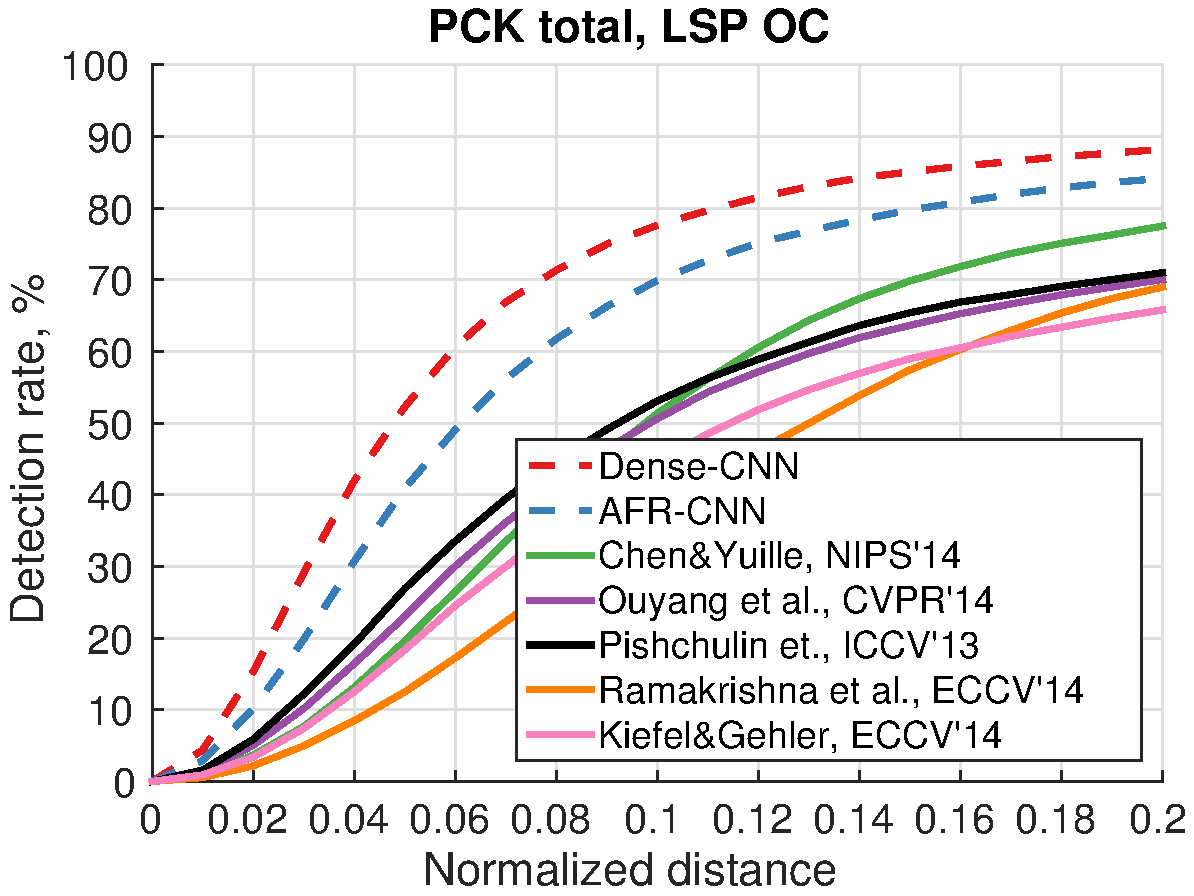
\includegraphics[width=0.6\linewidth]{pck-total-lsp-OC.pdf}&
  \end{tabular}
  %\vspace{-1.0em}
%  \caption{Pose estimation performance on (a) LSP (PC) dataset (PCK) and (b) MPII Single Person dataset (PCKh).} 
  \caption{Pose estimation results over all PCK thresholds on LSP (OC) dataset.} 
  \vspace{0.2em}
  \label{fig:pck-curves:lsp:oc}
   \vspace{-1.0em}
\end{figure}


Comparing the performance by $\rcnn$ and $\dense$ to the state of the
art, we observe that both proposed approaches significantly outperform
other methods. Both deep learning based approaches of
Chen\&Yuille~\cite{chen14nips} and Ouyang et al.~\cite{ouyang14cvpr}
are outperformed by $+10.7$ and $+18.2$\% PCK when compared to the
best performing $\dense$. Analysis of PCK curve for the entire range
of PCK distance thresholds reveals even larger performance differences
(c.f. Fig.~\ref{fig:pck-curves:lsp:oc}). The results using OC
annotations confirm our findings from PC evaluation and clearly show
the advantages of the proposed part detection models over the
state-of-the-art deep learning methods~\cite{chen14nips,ouyang14cvpr},
as well as over earlier pose estimation methods based on hand-crafted
image features~\cite{pishchulin13iccv,kiefel14eccv,ramakrishna14eccv}.

%\renewcommand{\tabcolsep}{0.15cm}
\tabcolsep 1.5pt
\begin{table}[tbp]
 \scriptsize
  \centering
  \begin{tabular}{@{} l cc ccc ccc@{}}
    \toprule
    &Torso & Upper & Lower & Upper & Fore- & Head  & PCP \\
    &   & Leg   & Leg& Arm   & arm   &       &       \\
    \midrule
%%     $\rcnn$ (unary) & 93.2  & 82.7  & 77.7  & 75.5  & 63.5  & 91.2 & 78.3 \\



%%     \quad+ $\deepcut$ \singb & 93.3  & 83.2  & 77.8  & 76.3  & 63.7  & 91.5 & 78.7 \\


%%     \quad\quad+ appearance pairwise & 93.4  & 83.5  & 77.8  & 76.6  & 63.8  & 91.8 & 78.9 \\

%%     \quad+ $\deepcut$ \multb & 93.6  & 83.3  & 77.6  & 76.3  & 63.5  & 91.2 & 78.6 \\

 
    $\rcnn$ (unary) & 92.9  & 86.3  & 79.8  & 77.0  & 64.2  & 91.8 & 79.9 \\   
    \midrule
    $\dense$ (unary)          & \textbf{96.0}  & \textbf{91.0}  & \textbf{83.5}  & \textbf{82.8}  & \textbf{71.8}  & \textbf{96.2} & \textbf{85.0} \\
    \midrule
    Chen\&Yuille~\cite{chen14nips}& 92.7  & 82.9  & 77.0  & 69.2  & 55.4  & 87.8 & 75.0 \\
    Ouyang et al.~\cite{ouyang14cvpr}& 88.6  & 77.8  & 71.9  & 61.9  & 45.4  & 84.3 & 68.7 \\
    Pishchulin et.~\cite{pishchulin13iccv}& 88.7  & 78.9  & 73.2  & 61.8  & 45.0  & 85.1 & 69.2 \\
    Kiefel\&Gehler~\cite{kiefel14eccv}& 84.3  & 74.5  & 67.6  & 54.1  & 28.3  & 78.3 & 61.2 \\
    Ramakrishna et al.~\cite{ramakrishna14eccv}& 88.1  & 79.0  & 73.6  & 62.8  & 39.5  & 80.4 & 67.8 \\
    \bottomrule
  \end{tabular}
  \caption[]{Pose estimation results (PCP) on LSP (OC) dataset.}
    \vspace{-1.5em}
  \label{tab:multicut:lsp-oc-pcp}
\end{table}


\myparagraph{PCP evaluation measure.} Results using OC annotations and
PCP evaluation measure are shown in
Tab.~\ref{tab:multicut:lsp-oc-pcp}. Overall, the trend is similar to
PC evaluation: both proposed approaches significantly outperform
the state-of-the-art methods with $\dense$ achieving the best result
of 85.0\% PCP thereby improving by $+10$\% PCP over the best
published result~\cite{chen14nips}.
